\documentclass{article}
\usepackage[utf8]{inputenc}
\usepackage{amsmath}
\usepackage[ruled,vlined]{algorithm2e}
\usepackage{graphicx}
\graphicspath{ {./images/} }

\title{A Semi-supervised Method for Training Deep Neural Networks}
\author{Misha Klopukh, Michael Teti, Elan Barenholtz, William Hahn}
\date{March 2019}

\begin{document}

\maketitle




\section{Abstract}

\section{Main}

Deep Convolutional Networks trained by gradient descent have become the standard for computer vision. This approach has become popular because of the high accuracy and relatively fast training with gradient descent.\cite{something} However, there are a several fundamental flaws in how we train these networks. An image classification task can be thought of as two tasks, detection -- where image features are identified -- and classification -- where a class is decided based on detected features. These tasks in theory are separate -- you shouldn't need to change your definition of an edge or corner to learn what a cat is.\cite{something} However, in modern deep learning, we allow the network to learn its primitive features while it is learning the task. This is done because we ourselves do not know what primitive features we need to best classify objects. Features learned by gradient descent have long been shown to outperform hand-designed features.\cite{something} However, learning these features slows down training significantly, as loss back-propagates through to the first layers and changes them often, even though the layers may have accurate features. This also causes the networks to learn more biases in the training data, and to require more data in order to learn more weights. Other problems with back-propagating through the entire network that arise more in larger networks include the vanishing gradient problem, which causes gradients at the beginning of the network to all be near zero and makes them unable to train properly.\cite{something} We propose a new way of training a neural network that mitigates these and other problems.
\newline
\begin{figure}
    \centering
    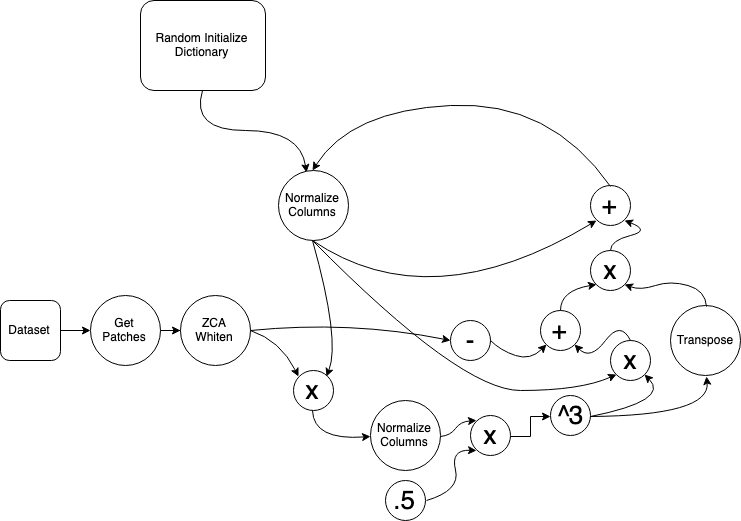
\includegraphics[width=.8\linewidth]{XCubed_diagram}
    \caption{Diagram of XCubed algorithm}
    \label{fig:diagram}
\end{figure}
\begin{figure}
    \centering
    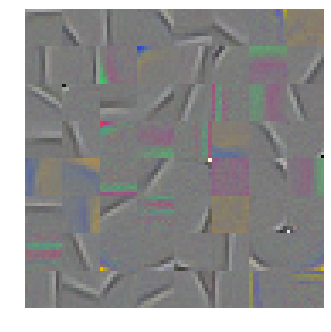
\includegraphics[width=.8\linewidth]{x3filters}
    \caption{Filters produced by XCubed}
    \label{fig:x3weights}
\end{figure}
\begin{figure}
    \centering
    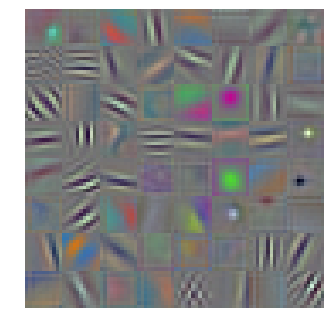
\includegraphics[width=.8\linewidth]{trainedfet}
    \caption{Filters learned by Alexnet's first layer}
    \label{fig:learnedweights}
\end{figure}
XCubed is an unsupervised, gradient-free, and loss-free algorithm for getting weights for a convolutional neural network. The algorithm, shown in Figure \ref{fig:diagram}, creates a dictionary of features from patches of your data using a repeated compounding method. When run on the Oxford 17 flowers dataset, the XCubed algorithm produces the first layer filters shown in Figure \ref{fig:x3weights} after 1000 iterations. Alexnet produces very similar filters, shown in figure \ref{fig:learnedweights}, but runs much longer, taking 2.5 hours on GPU rather than 3 seconds on CPU.
\section{Results}
\begin{figure}
    \centering
    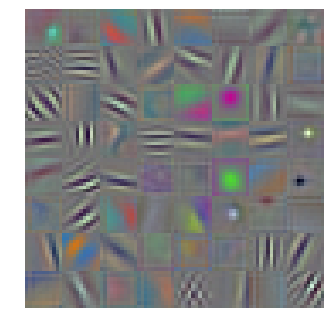
\includegraphics[width=.8\linewidth]{trainedfet}
    \caption{Filters learned by Alexnet's first layer}
    \label{fig:netspeedup}
\end{figure}
\section{Discussion}
\section{Methods}
\section{Additional information}
\section{Data availability}
\section{References}
\section{Acknowledgements}
\section{Author information}
\section{Supplementary information}
\section{Rights and permissions}
\section{About this article}




\end{document}